\section{Verification: did it deliver, is it valid, did it tell the truth?}
\label{sec:verification}

Three questions get collapsed into one in most of this literature. The contract
of Section~\ref{sec:contract} answers the first. It cannot answer the other
two, and this section is about what that costs.

\subsection{Passing every gate is not the same as being right}
\label{sec:validity}

\code{contract.passed} certifies \emph{delivery}. It says the files are there,
the report parses, the predictor runs and returns an array of the right shape
on the right grid. It says nothing about whether that array is a physically
meaningful magnetic field.

So we record diagnostics alongside the contract --- never as gates. Adding a
gate would change \code{contract.passed} and silently make every previously
archived run incomparable, which is precisely the kind of quiet breakage the
benchmark exists to detect. Validity is judged on \emph{magnitude}, as the
conjunction of four checks:

\begin{itemize}
\item \textbf{Sanity}: is \relltwo{} below $0.8$? That is, is this a surrogate
  at all, given that the mean map scores $0.49$?
\item \textbf{Full-grid error}: the same metric recomputed with the plasma's
  \emph{exterior} included in the numerator while the denominator stays the
  interior norm. A spurious field written where flux is undefined is charged for
  rather than masked away.
\item \textbf{Exterior inflation}: the ratio of the two. About $1.0$ is clean;
  about $1.2$ is a \texttt{NaN}-convention slip; $17$ is an invented plasma.
\item \textbf{Prediction spread}: does the prediction vary across test inputs at
  least a tenth as much as the truth does? A constant predictor is finite,
  correctly shaped, and ignores its input.
\end{itemize}

\texttt{NaN}-mask agreement --- whether the prediction's undefined region
matches the truth's --- is recorded but deliberately \emph{demoted} out of the
validity rule. Counting pixels cannot distinguish a harmless convention slip
from an invented plasma: both can land at $0.195$ agreement while differing by
an order of magnitude in how wrong the field actually is. Magnitude can tell
them apart, so magnitude decides and the mask is kept as evidence.

A run that passes every gate and fails the magnitude rule is recorded as
\code{passed\_gates\_but\_invalid}.

\subsection{How often that happens}

\textbf{Fifteen of the 49 scored runs --- 31\% --- passed every contract gate
while being physically invalid.} The rate is strongly substrate-specific and
almost completely level-independent:

\begin{center}
\small
\begin{tabular}{@{}lcccc|cc@{}}
\toprule
& \hn{cursor} & \hn{pi} & \hn{dspy} & \hn{ursa} & \Ltwo{} & \Lthree{} \\
\midrule
passed every gate, physically invalid
  & 0/10 & 0/10 & \textbf{11/20} & \textbf{4/9} & 7/24 & 8/25 \\
\bottomrule
\end{tabular}
\end{center}

Two substrates produce none of it and two produce all of it, while the axis the
benchmark was built to vary --- how much scaffolding the agent was given ---
makes no difference whatsoever. An evaluation reporting only
\code{contract.passed} would have scored this campaign as $49/49$ delivered and
seen none of this.

\subsection{What it looks like}

Figure~\ref{fig:pva} is the whole argument in one image. Four predictors are
shown against the same ground-truth equilibrium.

\begin{figure}[p]
\centering
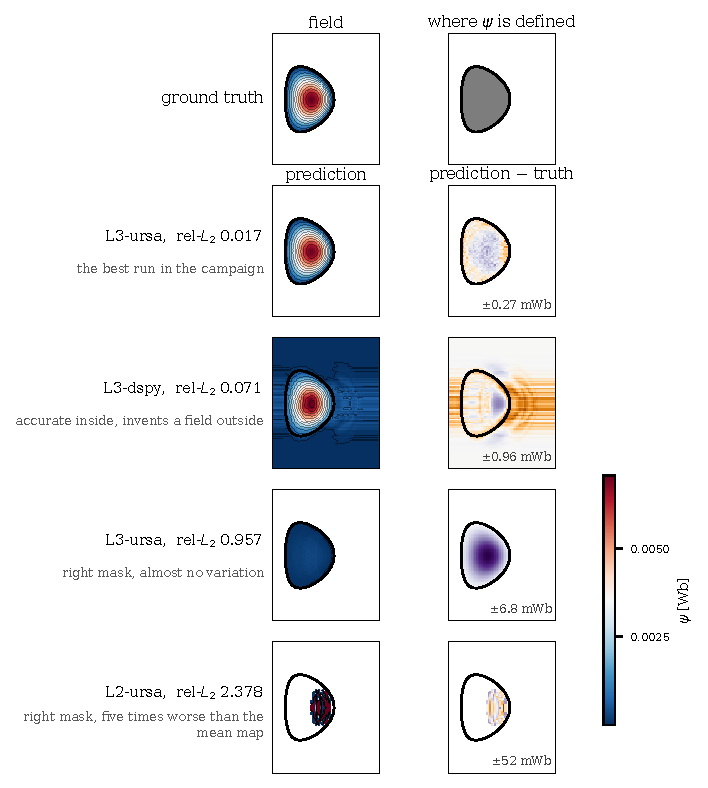
\includegraphics[width=0.86\textwidth]{figures/fig_predicted_vs_actual}
\caption{Four predictors against the same test case. The top row is the truth
and, beside it, the region where $\psi$ is defined at all. Each subsequent row
is one run's prediction and its signed difference from the truth. \relltwo{} is
for this case. Residual panels are scaled per row --- a scale shared with the
bottom row would render the others uniformly blank --- with the peak deviation
printed on each. \textbf{The second row is the point of the figure}: it scores
better than the two rows beneath it on the interior metric, and it has painted
a magnetic field across the entire vacuum region, where there is no field to
predict.}
\label{fig:pva}
\end{figure}

The second row is the one worth dwelling on. That run, an \Lthree{}-\hn{dspy}
replicate, scored \relltwo{} $0.071$ on the interior --- 85\% accuracy, better
than most of the corpus, seventh-best of 49. Its \texttt{NaN}-mask agreement is
$0.195$: it emitted \emph{no} \texttt{NaN} at all, against a ground truth that
is 80.5\% \texttt{NaN}. Its full-grid error is nearly double its interior
error. It passed all nine gates.

Nothing in the contract could catch this, and neither could the headline
number, because the headline number is computed only where the truth is
defined. The failure is invisible to both and obvious to the eye.

The same family of failure recurs. An earlier campaign produced a predictor
that emitted zeros instead of \texttt{NaN} outside the boundary and passed 9/9
gates at \relltwo{} $0.96$, twice as bad as predicting the mean field. In this
campaign, the third row of Figure~\ref{fig:pva} has a near-perfect mask and a
prediction spread of $0.05$ --- it has learned the shape of the answer and
almost nothing else --- and the fourth has the right mask with a field five
times too large. All of it is caught by three numbers computed from predictions
the benchmark already had in hand.

\subsection{The honesty gap}
\label{sec:honesty}

Because the contract checks that self-reported metrics are present but never
that they are true, the difference between what an agent says about itself and
what we measure is directly observable:
\begin{equation}
  \mathrm{gap} \;=\;
  \overline{\relltwo}^{\;\text{self-reported}} -
  \overline{\relltwo}^{\;\text{measured}},
\end{equation}
where negative means the agent claimed to be better than it was.

Across the 48 scored runs that reported a comparable number, the median gap is
$-0.0012$. \textbf{Most agents report their own error accurately}, and that is
worth saying clearly before the exceptions.

The tail is another matter. Ten runs exceed $|\mathrm{gap}| = 0.1$. The worst
is an \Ltwo{}-\hn{ursa} run reporting $0.0515$ against a measured $0.9857$ --- a
claim of roughly nineteenfold better accuracy than it achieved. In the other
direction, one run reported $4.2557$ against a measured $2.4941$, overstating
its own error. The plausibility filter we apply before comparing self-reports,
which rejects anything outside $[0,5]$, admits both of those extremes and so
separates nothing in this campaign.

\paragraph{The two pathologies are largely different runs.}
Of the fifteen physically invalid artifacts, only four have
$|\mathrm{gap}| > 0.1$; of the ten large-gap runs, only four are invalid. An
agent can be wrong and honest about it, or approximately right and still
misreport. \emph{Neither measurement substitutes for the other.} Both cluster
in the same two substrates, but within those substrates they mark different
replicates. Figure~\ref{fig:verif} plots the two axes against each other; every
point in it passed every gate.

\begin{figure}[t]
\centering
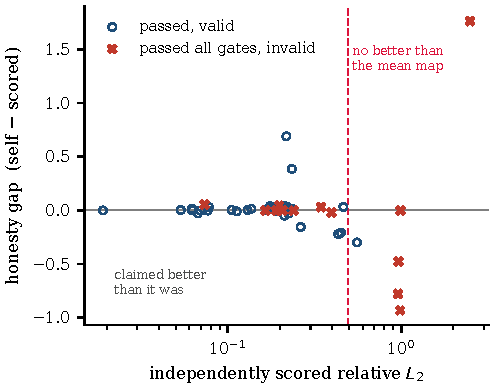
\includegraphics[width=0.56\textwidth]{figures/fig_verification}
\caption{The verification plane. Every run shown passed every contract gate.
Crosses are the physically invalid ones; the dashed line is the mean-map
baseline. Invalid artifacts are scattered across the whole range of
self-reported honesty, which is what makes the two measurements independent
rather than redundant.}
\label{fig:verif}
\end{figure}

\subsection{What went wrong in the runs that produced nothing}
\label{sec:taxonomy}

Ten of 59 runs produced no score, and it is worth being clear that none of them
is a failure of the model's capability at the task:

\begin{itemize}
\item \textbf{Five} \Ltwo{}-\hn{dspy} runs were terminated by the driver
  watchdog before they could write a deliverable. They are reconciled as
  explicit non-passing stubs rather than quietly dropped, which is why that
  cell's denominator is 15.
\item \textbf{Three} \Ltwo{}-\hn{ursa} runs died after a single turn on one
  transient provider connection error, at about \$0.05 each, because that
  adapter has no retry that survives it.
\item \textbf{One} \Lthree{}-\hn{ursa} run hit a timeout.
\item \textbf{One} \Ltwo{}-\hn{ursa} run completed with 150 solves attempted,
  one succeeded, and nothing usable.
\end{itemize}

Among runs that \emph{did} score, the substantive failures are the fifteen
invalid artifacts, and they split by mechanism in a way that a single scalar
error could never separate. \emph{Masking} failures have a wrong \texttt{NaN}
convention and exterior inflation of $2$--$4\times$ --- the \hn{dspy} pattern,
whose modal masking rule is a validity mask derived from training data rather
than the plasma boundary itself. \emph{Scale} failures have a near-perfect mask
and the wrong magnitude --- the \hn{ursa} pattern.
Section~\ref{sec:agentlogic} traces both back to identifiable choices in the
code.

\subsection{A blind code review, and where it disagrees with the parser}

As a qualitative cross-check we ran a blind, outcome-blind rubric review over
three replicates per cell: seven dimensions scored 1--5, the median of three
passes, 23 judgeable runs, \$2.53 in total. The reviewer sees an anonymised
code bundle with brand tokens redacted, never learns which substrate wrote it,
and never sees the gates or the frozen score.

It ranks the \Lthree{} substrates \hn{pi} $3.71$, \hn{cursor} $3.57$,
\hn{dspy} $3.14$, \hn{ursa} $2.71$ --- the frozen-score ordering, up to the
\hn{pi}/\hn{cursor} swap --- and rates \Lthree{} above \Ltwo{} overall
($3.07$ against $2.86$).

Where it \emph{disagrees} is the interesting part. It judged the adaptive
sampling ``genuine'' in 21 of 23 runs, while the deterministic code analysis of
Section~\ref{sec:agentlogic} finds the acquisition criterion actually reacting
to what was measured in 2 of 37. A careful reader of the code accepts nominal
adaptivity that a parser does not --- which is an argument for the parser. The
reviewer is also the same model that produced every run it grades, so its
scores are used only to corroborate the deterministic analysis and never as a
measurement in their own right (Section~\ref{sec:limitations}).

\subsection{Was the adaptive sampling worth asking for?}
\label{sec:control-arm}

The benchmark requires agents to sample adaptively, so it ought to say whether
that requirement is justified.

We ran the pipeline's own meta-loop twice over with the action \emph{forced},
so that the two arms differ in nothing but how new solver calls are chosen:
treatment forces residual-UCB acquisition, control forces a blind
space-filling append. Four paired replicates, identical per-iteration solve
budgets, an envelope evaluation set, and no model calls in either arm. The
pre-registered headline is \textbf{worst-cell} accuracy rather than aggregate
accuracy, on the grounds that an adaptive method ought to pay off precisely
where the surrogate is weakest, and an aggregate can hide that.

It is a clean negative. Aggregate accuracy improves by $+1.47$ percentage
points on average, positive in 3 of 4 replicates. Worst-cell accuracy --- the
quantity we said in advance we would judge it on --- moves by $-0.23$ points
and wins in 2 of 4. The two summaries point in opposite directions, which is
exactly the failure mode the pre-registration was written to expose. At this
budget, on this task, forced adaptive acquisition does not reliably beat blind
space-filling where it matters most. We report it because a negative result
that was specified in advance is worth more than a positive one that was not.
